\newtheorem{proposition}{Proposition}
\newtheorem{lemma}{Lemma}
\newtheorem{assumption}{Assumption}

\chapter{Flexible Diffusion on Varying Dimensionality Data}
\label{ch:tddm}

So far in this thesis we have described how to train a diffusion model to be flexibly conditioned on any subset of its dimensions at test time, and how to adapt such a model to high-dimensional video data with bounded compute resources. In this section we explore how to enable flexible conditioning in another scenario: when the data $\rvx$ that we wish to infer has unknown dimensionality. This can be an issue with molecular data, where the number of atoms could vary, or with video data, where the number of frames can vary. When defining a generative model over these data-types, it is necessary to model the number of dimensions along with the raw values of each of its dimensions (the state). Previous approaches to modelling such data have relied on first sampling the number of dimensions from the empirical distribution obtained from the training data, and then sampling data using a fixed dimension diffusion model (FDDM) conditioned on this number of dimensions~\cite{hoogeboom2022equivariant}. This works well for unconditional generative modelling. For conditional modelling, where the number of dimensions may depend on the observations, this approach does not apply and we are forced to first train an auxiliary model that predicts the number of dimensions given the observations~\cite{igashov2022equivariant}.

This approach to trans-dimensional generative modelling is fundamentally limited due to the complete separation of dimension generation and state value generation. A particular limitation is in the common use-case of conditional sampling from an unconditional diffusion model discussed in \cref{sec:other-methods-for-conditional-sampling}. Here, an unconditional diffusion model is trained that end-users can then easily and cheaply adapt to their task of interest through conditioning~\cite{song2020score, dhariwal2021diffusion, clip_guided_diffusion, zhang2023towards} without needing to perform any further training or fine-tuning of the model. In an FDDM, there is no way for the guidance to appropriately guide the dimension of the generated datapoint. This can lead to incorrect generations for datasets where the dimension greatly affects the nature of the datapoint created, which is common since e.g. small molecules have completely different properties to large molecules.

To generate data of varying dimensionality, we propose a jump diffusion based generative model that jointly generates both the dimension and the state. Our model can be seen as a unification of diffusion models which generate all dimensions in parallel with autoregressive type models which generate dimensions sequentially. We derive the model through constructing a forward noising process that adds noise and removes dimensions and a backward generative process that adds dimensions while removing noise. We depict both processes in \cref{fig:tddm-fig1}. We derive the optimum backward generative process as the time-reversal of the forward noising process and derive a novel learning objective to learn this backward process from data. We demonstrate the advantages of our method on molecular and video datasets finding our method achieves superior guided generation performance and produces more representative data interpolations across dimensions.

\begin{figure}
    \centering
    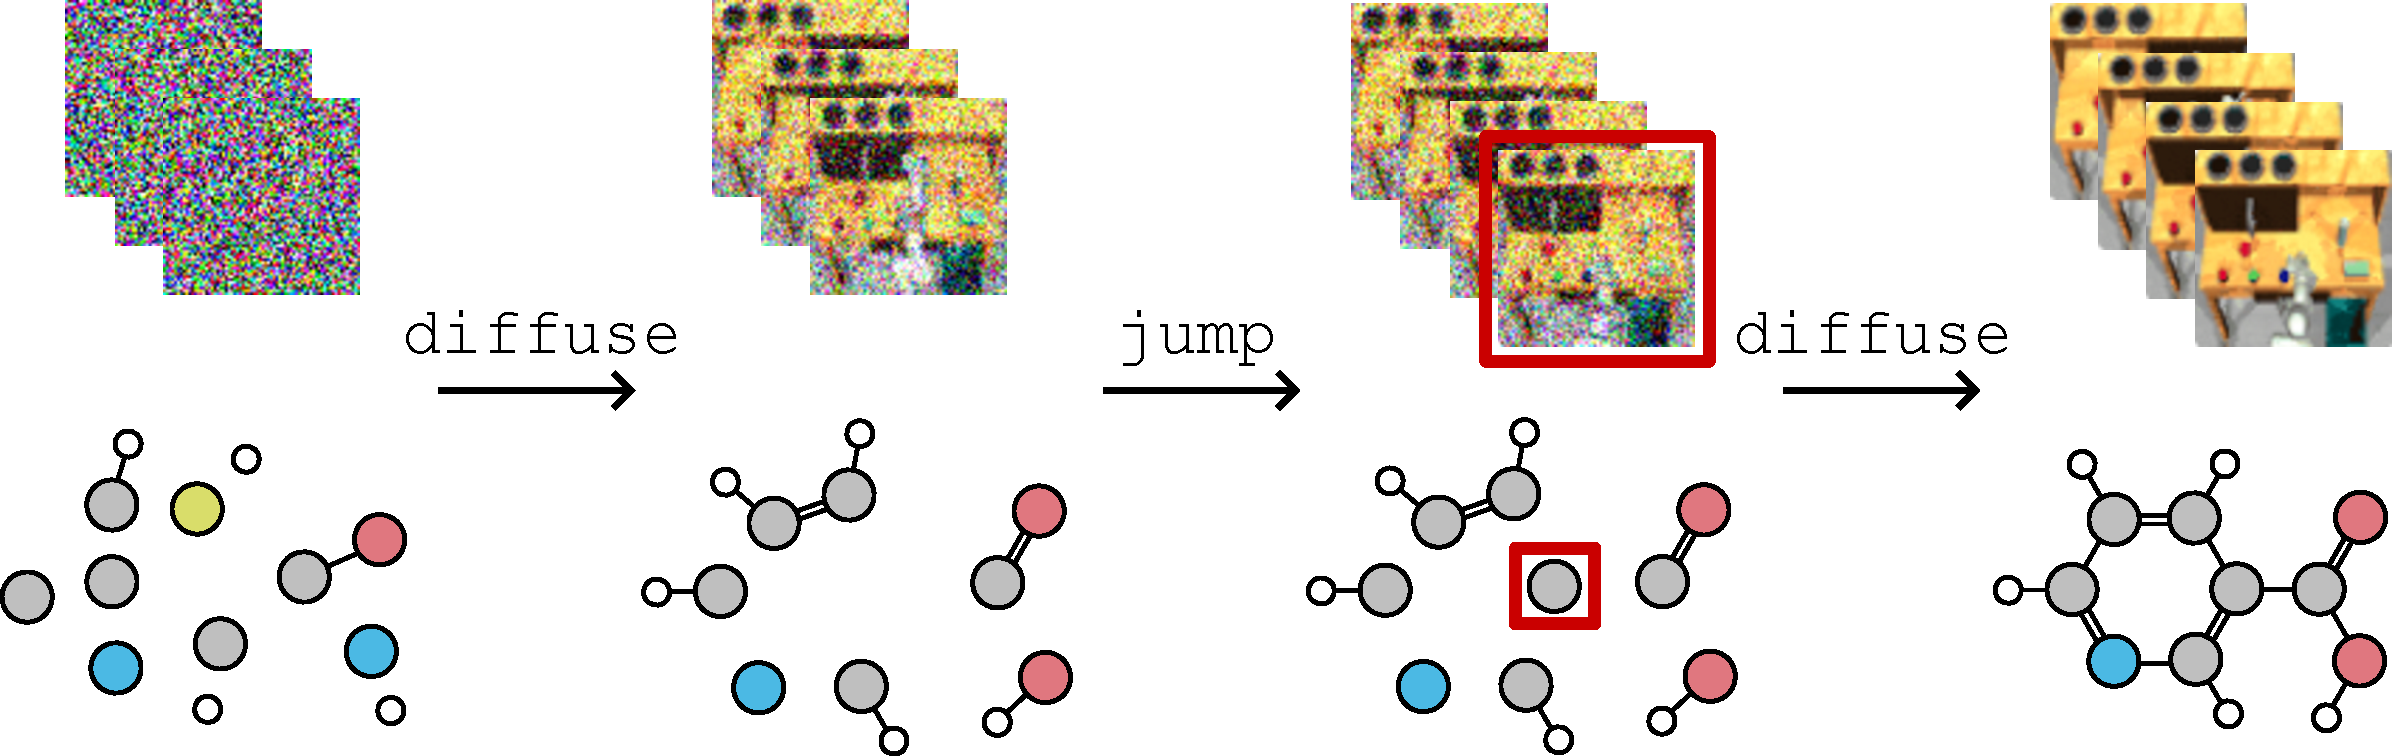
\includegraphics[width=\textwidth]{figs/tddm/fig1.pdf}
    \caption{Illustration of the jump diffusion generative process on videos and molecules. The generative process consists of two parts: a diffusion part which denoises the current set of frames/atoms and a jump part which adds on a suitable number of new frames/atoms such that the final generation is a clean synthetic datapoint of an appropriate size.
    }
    \label{fig:tddm-fig1}
\end{figure}


% \section{Background}
% Standard continuous-time diffusion models \cite{song2020score,huang2021variational,karraselucidating2022,benton2022denoising}  define a forward diffusion process through a stochastic differential equation (SDE) where $\rvx_0 \sim \pdata$ and, for $t>0$,
% \begin{equation}\label{eq:forwardnoising}
%      \rmd \rvx_t = \rvb_t(\rvx_t) \rmd t + \diffcoeff_t \rmd \brown_t,
% \end{equation}
% where $\rvx_t \in \mathbb{R}^d$ is the current state, $\rvb_t: \mathbb{R}^d \rightarrow \mathbb{R}^d$ is the drift and $\diffcoeff_t \in \mathbb{R}$ is the diffusion coefficient. $ \rmd \brown_t$ is a Brownian motion increment on $\mathbb{R}^d$. This SDE can be understood intuitively by noting that in each infinitesimal timestep, we move slightly in the direction of the drift $\rvb_t$ and inject a small amount of Gaussian noised governed by $\diffcoeff_t$.
% Let $p_t(\rvx_t)$ denote the distribution of $\rvx_t$ for the forward diffusion process \eqref{eq:forwardnoising} so that $p_0(\rvx_0) = \pdata(\rvx_0)$. $\rvb_t$ and $\diffcoeff_t$ are set such that at time $t=T$, $p_T(\rvx_T)$ is close to $\pref(\rvx_T)= \mathcal{N}(\rvx_T;0, I_d)$; e.g. $\rvb_t(\rvx_t)=-\frac{1}{2}g(t)^2 \rvx_t,$ for $g(t)>0$ \cite{ho2020denoising, song2020score}.

% The time-reversal of the forward diffusion \eqref{eq:forwardnoising} is also a diffusion \cite{anderson1982reverse, haussmann1986time} which runs backwards in time from $p_T(\rvx_T)$ to $p_0(\rvx_0)$ and satisfies the following reverse time SDE
% \begin{equation}
%      \rmd \rvx_t = \backwarddrift_t(\rvx_t) \rmd t + \diffcoeff_t \rmd \hat{\brown}_t,
% \end{equation}
% where $\backwarddrift_t(\rvx_t) = \rvb_t(\rvx_t) - \diffcoeff_t^2 \nabla_{\rvx_t} \log p_t(\rvx_t)$, $\rmd t$ is a negative infinitesimal time step and $\rmd \hat{\brown}_t$ is a Brownian motion increment when time flows backwards. 
% Unfortunately, both the terminal distribution, $p_T(\rvx_T)$, and the score, $\nabla_{\rvx_t} \log q(\rvx_t)$, are unknown in practice.
% A generative model is obtained by approximating $p_T$ with $\pref$ and learning an approximation $s^\theta_{t}(\rvx_t)$ to $\nabla_{\rvx_t} \log q(\rvx_t)$ typically using denoising score matching \cite{vincent2011connection}, i.e. 
% \begin{equation}
%     \underset{\theta}{\text{min}} \quad \mathbb{E}_{\mathcal{U}(t; 0, T) q(\rvx_0, \rvx_t)} [ \norm{s^\theta_t(\rvx_t) - \nabla_{\rvx_t} \log p_{t|0}(\rvx_t | \rvx_0)}^2 ].
%     \label{eq:dsm}
% \end{equation}
% For a flexible model class, $s^\theta$, we get $s^\theta_t(\rvx_t) \approx \nabla_{\rvx_t} \log p_t(\rvx_t)$ at the minimizing parameter.

\section{Trans-Dimensional Generative Model}
Instead of working with fixed dimension datapoints, we will instead assume our datapoints consist of a variable number of components. A datapoint $\mX$ consists of $n$ components each of dimension $d$. For ease of notation, each datapoint will explicitly store both the number of components, $n$, and the state values, $\rvx$, giving $\mX = (n, \rvx)$. Since each datapoint can have a variable number of components from $n=1$ to $n=N$, our overall space that our datapoints live in is the union of all these possibilities, $\mX \in \gX = \bigcup_{n=1}^N \{n \} \times \mathbb{R}^{nd}$. For example, for a varying size point cloud dataset, components would refer to points in the cloud, each containing $(x,y,z)$ coordinates giving $d=3$ and the maximum possible number of points in the cloud is $N$.

Broadly speaking, our approach will follow the same framework as previous diffusion models. We will first define a forward noising process that both corrupts state values with Gaussian noise and progressively deletes dimensions.
We then learn an approximation to the time-reversal giving a backward generative process that simultaneously denoises whilst also progressively adding dimensions back until a synthetic datapoint of appropriate dimensionality has been constructed.

\subsection{Forward Process}
\label{sec:tddm-jump-diff-proc}

Our forward and backward processes will be defined through jump diffusions. A jump diffusion process has two components, the diffusion part and the jump part. Between jumps, the process evolves according to a standard SDE. When a jump occurs, the process transitions to a different dimensional space with the new value for the process being drawn from a transition kernel $K_t(\mV | \mX): \gX \times \gX \rightarrow  \mathbb{R}_{\geq 0}$. Letting $\mV = (m, \rvy)$, the transition kernel satisfies $\sum_m \int_\rvy K_t(m, \rvy | \mX) \rmd \rvy = 1$ and $\int_\rvy K_t(m=n, \rvy | \mX) \rmd \rvy = 0$. The rate at which jumps occur (jumps per unit time) is given by a rate function $\lambda_t(\mX): \mathcal{X} \rightarrow \mathbb{R}_{\geq 0}$. 
We can describe a jump diffusion in terms of an infinitesimal timestep $\rmd t$. For the forward process we call the transition kernel $\ftk_t(\mV|\mX)$ and rate function $\forwardrate_t(\mX_t)$. We will give their precise definitions shortly. Given this notation, we write the forward jump diffusion as
\begin{align}
    \textbf{Jump} \hspace{1cm} & \mX_t' = \begin{cases}
        \mX_t & \text{with probability } 1 - \forwardrate_t(\mX_t) \rmd t \\
        \mV \sim \ftk_t( \mV |\mX_t) & \text{with probability } \forwardrate_t(\mX_t) \rmd t
    \end{cases}  \label{eq:tddm-forward-jump} \\
    \textbf{Diffusion} \hspace{1cm} &\rvx_{t+ \rmd t} = \rvx'_t + \rvb_t(\rvx'_t) \rmd t + g(t) \rmd \brown_t \hspace{1cm} n_{t+\rmd t} = n_t'
     \label{eq:tddm-forward-diffusion}
\end{align}
with $\mX_t \triangleq (n_t, \rvx_t)$ and $\mX_{t+\rmd t} \triangleq (n_{t+\rmd t}, \rvx_{t + \rmd t})$ and $\rmd \brown_t$ being a Brownian motion increment on $\mathbb{R}^{n_t'd}$. We provide a more formal definition in \cref{sec:tddm-Proofs}.

With the jump diffusion formalism in hand, we can now construct our forward noising process. We will use the diffusion part to corrupt existing state values with Gaussian noise and the jump part to destroy dimensions. For the diffusion part, we use the variance-preserving diffusion SDE introduced in \cref{ch:diffusion}~\cite{ho2020denoising, song2020score} so $\rvb_t(\rvx_t) = -\frac{1}{2}g(t)^2 \rvx_t$.

When a jump occurs in the forward process, one component of the current state will be deleted.
For example, one point in a point cloud or a single frame in a video is deleted. The rate at which these deletions occur is set by a user-defined forward rate $\smash{\forwardrate_t}(\mX)$. To formalise the deletion, we need to introduce some more notation. We let $\delidxdist(i | n)$ be a user-defined distribution over which component of the current state to delete. We also define $\text{del}: \mathcal{X} \times \mathbb{N} \rightarrow \mathcal{X}$ to be the deletion operator that deletes a specified component. Specifically, $(n-1, \rvy) = \text{del}((n, \rvx), i)$ where $\rvy \in \mathbb{R}^{(n-1)d}$ has the same values as $\rvx \in \mathbb{R}^{nd}$ except for the $d$ values corresponding to the $i$th component which have been removed. 
We can now define the forward jump transition kernel as $\ftk_t(\mV | \mX) = \sum_{i=1}^n \delidxdist (i | n) \updelta_{\text{del}(\mX, i)}(\mV)$. We note that only one
component is ever deleted at a time meaning $\ftk_t(m, \rvy | \mX) = 0$ for $m \neq n - 1$. Further, the choice of $\delidxdist(i | n)$ will dictate the behaviour of the reverse generative process. If we set $\delidxdist(i | n) = \mathbb{I}\{i=n\}$ then we only ever delete the final component and so in the reverse generative direction, datapoints are created additively, appending components onto the end of the current state. Alternatively, if we set $\delidxdist(i | n) = 1/n$ then components are deleted uniformly at random during forward corruption and in the reverse generative process, the model will need to pick the most suitable location for a new component from all possible positions.

The forward noising process is simulated from $t=0$ to $t=T$ and should be such that at time $t=T$, the marginal probability $p_t(\mX)$ should be close to a reference measure $\pref(\mX)$ that can be sampled from. 
We set $\pref(\mX) = \mathbb{I} \{ n = 1\} \mathcal{N}(\rvx; 0, I_{d})$ where $\mathbb{I} \{ n = 1\}$ is $1$ when $n=1$ and $0$ otherwise. To be close to $\pref$, for the jump part, we set $\forwardrate_t$ high enough such that at time $t=T$ there is a high probability that all but one of the components in the original datapoint have been deleted. For simplicity, we also set $\forwardrate_t$ to depend only on the current dimension $\forwardrate_t(\mX) = \forwardrate_t(n)$ with $\forwardrate_t(n=1) = 0$ so that the forward process stops deleting components when there is only $1$ left. In our experiments in \cref{sec:tddm-experiments} we demonstrate the trade-offs between different rate schedules in time. For the diffusion part, we use standard $g(t)$ schedules which ensure that we are close to $\mathcal{N}(\rvx; 0, I_{d})$.

\subsection{Backward Process}
The backward generative process will simultaneously denoise and add dimensions back in order to construct the final datapoint. Its drift term corresponds to that of a standard reverse diffusion SDE from \cref{ch:diffusion}, consisting of the sum of the forward drift term and a scaled score function. We will call the backwards rate function $\backwardrate_t(\mX)$, the backwards transition kernel $\btk_t(\mV | \mX)$, the backwards drift term $\backwarddrift(\mX)$ and the backwards diffusion coefficient $\backwarddiffcoeff_{t}$ so write the backwards jump diffusion as
\begin{align}
    \label{eq:tddm-reverse-jump}
    \textbf{Jump} \hspace{.4cm} & \mX_t' = \begin{cases}
        \mX_t & \text{with probability } 1 - \backwardrate_t(\mX_t) \rmd t \\
        \mV \sim \btk_t( \mV |\mX_t) & \text{with probability } \backwardrate_t(\mX_t) \rmd t
    \end{cases} 
    \\
    \label{eq:tddm-reverse-diffusion}
    \textbf{Diffusion} \hspace{.4cm} &\rvx_{t+ \rmd t} = \rvx'_t + \backwarddrift(\rvx'_t)
    % \left(b(t)\rvx_t + g(t)^2 \rvs_\theta(\mX, t) \right) 
    \rmd t + \backwarddiffcoeff(t) \rmd \brown_t \hspace{.5cm} n_{t+\rmd t} = n_t'
\end{align}
We would now like to specify the form of $\backwardrate_t(\mX)$, $\btk(\mV|\mX)$, and $\backwarddrift(\mX)$ which ensure that the backward process is the time-reversal of the forward process. 
% In order to find the time-reversal of the forward process, we must first introduce some notation to describe $\btk_t(\mV | \mX)$.
$\btk_t(\mV | \mX)$ should undo the forward deletion operation. Since $\ftk_t(\mV | \mX)$ chooses a component and then deletes it, $\btk_t(\mV | \mX)$ will need to generate the state values for a new component, decide where the component should be placed and then insert it at this location. 
Our new component will be denoted $\yadd \in \mathbb{R}^{d}$. 
The insertion operator is defined as $\text{ins}: \gX \times \mathbb{R}^{d} \times \mathbb{N} \rightarrow \gX$. It takes in the current value $\mX$, the new component $\yadd$ and an index $i \in \{1, \dots, n+1\}$ and inserts $\yadd$ into $\mX$ at location $i$ such that the resulting value $\mV = \text{ins}(\mX, \yadd, i)$ has $\text{del}(\mV, i) = \mX$.
We denote the joint conditional distribution over the newly added component and the index at which it is inserted as $\autonet_t(\yadd, i | \mX)$.
We therefore have $\btk_t(\mV | \mX) = \int_{\yadd} \sum_{i=1}^{n+1}  \autonet_t(\yadd, i | \mX) \updelta_{\text{ins}(\mX, \yadd, i)}(\mV) \rmd \yadd$. Noting that only one component is ever added at a time, we have $\btk_t(m, \rvy | \mX) = 0$ for $m \neq n+1$. 

This backward process formalism can be seen as a unification of diffusion models with autoregressive models. The diffusion part $\backwarddrift_t$ denoises the current set of components in parallel, whilst the autoregressive part $\autonet_t(\yadd, i | \mX)$ predicts a new component and its location. $\backwardrate_t(\mX)$ is the glue between these parts controlling when and how many new components are added during generation.

% \begin{table}
% \caption{Summary of forward and parameterized backward processes}
% \label{tab:forward_and_backward}
% \centering
% \small
% \begin{tabular}{@{}cccc@{}}
% \toprule
% Direction & $\drift_t$ & $\lambda_t(\mX)$ & $K_t(\mV | \mX)$ \\ \midrule
% \textbf{Forward} & $-\frac{1}{2} g(t)^2 \x$ & $\forwardrate_t(n)$ & $\sum_{i=1}^n \delidxdist(i | n) \updelta_{\text{del}(\mX, i)}(\mV)$ \\
% \textbf{Backward} & $ -\frac{1}{2} g(t)^2 \x - g(t)^2 s_{t}^\theta(\mX)$ & $\backwardrate_t^\theta(\mX)$ & $\int_{\yadd} \sum_{i=1}^{n+1}  \autonet^\theta_t(\yadd, i | \mX) \updelta_{\text{ins}(\mX, \yadd, i)}(\mV) \rmd \yadd$ \\ \bottomrule
% \end{tabular}
% \end{table}

The following proposition states the values for $\backwarddrift_t(\mX)$, $\backwarddiffcoeff_t(\mX)$, $\backwardrate_t(\mX)$ and $A_t(\yadd, i | \mX)$ which ensure that the backward process is the time-reversal of the forward process.
\begin{proposition}
\label{prop:time_reversal}
The time reversal of a forward jump diffusion process given by drift $b(t)$, diffusion coefficient $g(t)$, rate $\forwardrate_t(n)$ and transition kernel $\sum_{i=1}^n \delidxdist(i | n) \updelta_{\textup{del}(\mX, i)}(\mV)$ is given by a jump diffusion process with drift term $\backwarddrift$, diffusion coefficient $\backwarddiffcoeff_{t}^*$ and rate $\backwardrate_t^*(\mX)$ and transition kernel $\int_{\yadd} \sum_{i=1}^{n+1}  \autonet^*_t(\yadd, i | \mX) \updelta_{\textup{ins}(\mX, \yadd, i)}(\mV) \rmd \yadd$ as defined below
\begin{align}
    &\backwarddrift_{t}^*(\mX_t) = \rvb_{t}(\mX_t) - g_t^2 \nabla_{\rvx_t} \log q(\mX_t), \qquad \backwarddiffcoeff_{t}^* = g_{t},\\
    & \backwardrate_{t}^*(\mX_t) = \forwardrate_{t}(n+1) \frac{ \sum_{i=1}^{n+1} \delidxdist(i | n+1) \int_{\yadd} q_t(\textup{ins}(\mX_t, \yadd, i)) \rmd \yadd }{q(\mX_t)},\\
    & \autonet_{t}^*( \yadd, i | \mX) \propto q_{t}(\textup{ins}(\mX, \yadd, i) ) \delidxdist(i| n+1).
\end{align}
\end{proposition}
All proofs are given in \cref{sec:tddm-Proofs}. The expressions for $\backwarddrift_t^*$ and $\backwarddiffcoeff^*_t$ are the same as for a standard diffusion except for replacing $\nabla_{\rvx} \log p_t(\rvx)$ with $\nabla_{\rvx} \log p_t(\mX) = \nabla_{\rvx} \log p_t(\rvx | n)$ which is simply the score in the current dimension.
The expression for $\backwardrate_t^*$ can be understood intuitively by noting that the numerator in the probability ratio is the probability that at time $t$, given a deletion occurs, the forward process will arrive at $\mX$. If this is higher than the raw probability at time $t$ that the forward process is at $\mX$ (the denominator) then we should have high $\backwardrate_t^*$ because $\mX$ is likely the result of a deletion of a larger datapoint.
Finally the optimum $\autonet^*_t(\yadd, i | \mX)$ is simply the conditional distribution of $\yadd$ and $i$ given $\mX$ when the joint distribution over $\yadd, i, \mX$ is given by $p_{t}(\text{ins}(\mX, \yadd, i) ) \delidxdist(i| n+1)$. 

\subsection{Objective for Learning the Backward Process}
The true $\backwarddrift_t^*$, $\backwardrate_t^*$ and $\autonet_t^*$ are unknown so we need to learn approximations to them, $\backwarddrift_t^\theta$, $\backwardrate_t^\theta$ and $\autonet_t^\theta$. 
To parameterise the diffusion component of the reverse process, we can follow the procedure used in a standard diffusion model to learn the score function $\rvs_\theta(\mX, t) \approx \nabla_{\rvx_t} \log q(\mX_t)$. To parameterise the jump component, which relies on an unknown optimal rate $\backwardrate_t^*$ and unknown distribution $\autonet_t^*$, we will need a novel objective to learn approximations to $\backwardrate_t^\theta$ and $\autonet_t^\theta$.

As we showed in \cref{ch:diffusion}, the standard diffusion score matching loss can be derived from maximising an evidence lower bound on the model probability for $ \mathbb{E}_{\pdata(\rvx_0)} [ \log p_\theta(\rvx_0) ]$ \cite{song2021maximum}.
We derive here an equivalent loss to learn all of $\rvs_\theta$, $\smash{\backwardrate_t^\theta}$ and $\autonet_t^\theta$ for our jump diffusion process by leveraging the results of \cite{benton2022denoising} and \cite{cheridito2005equivalent}. Before presenting this loss, we first introduce some notation. Our objective for $s_\theta(\mX_t, t)$ will resemble denoising score matching (as in \cref{eq:exp-diffusion-loss-all-sigma} of \cref{sec:diffusion-training}) but instead involve the conditional score $\nabla_{\rvx_t} \log q(\mX_t | \mX_0) = \nabla_{\rvx_t} \log q(\rvx_t | \mX_0, n_t)$. This is difficult to calculate directly due to a combinatorial sum over the different ways the components of $\mX_0$ can be deleted to get to $\mX_t$. We avoid this problem by equivalently conditioning on a mask variable $M_t \in \{0, 1\}^{n_0}$ that is 0 for components of $\mX_0$ that have been deleted to get to $\mX_t$ and 1 for components that remain in $\mX_t$. This makes our denoising score matching target easy to calculate: $\nabla_{\rvx_t} \log q(\rvx_t | \mX_0, n_t, M_t) = \frac{\sqrt{\alpha_t} M_t(\rvx_0) - \rvx_t}{1 - \alpha_t}$ where $\alpha_t = \text{exp} ( - \int_{0}^t g(t)^2 \rmd s )$ \cite{song2020score}. Here $M_t(\rvx_0)$ is the vector removing any components in $\rvx_0$ for which $M_t$ is $0$, thus $M_t(\rvx_0)$ and $\rvx_t$ have the same dimensionality. We now state our full objective.

\begin{proposition}
\label{prop:elbo}
For the backward generative jump diffusion process starting at $\pref(\mX_T)$ and finishing at $ p_0^\theta(\mX_0)$, an evidence lower bound on the model log-likelihood $ \mathbb{E}_{\rvx_0 \sim \pdata} [ \log p_\theta(\rvx_0) ]$ is given by
\begin{align}
    \label{eq:elbo_line_1}
    \mathcal{L}(\theta) = -\frac{T}{2} \mathbb{E}\Big[& \diffcoeff_t^2 \norm{s_\theta(\mX_t, t) - \nabla_{\rvx_t} \log q(\rvx_t | \mX_0, n_t, M_t)   }^2 \Big] + \\
    \label{eq:elbo_line_2}
    T \mathbb{E} \Big[& - \backwardrate_{t}^\theta(\mX_t) + \forwardrate_t (n_t) \log \backwardrate_{t}^\theta(\mV) + \forwardrate_t(n_t) \log \autonet_{t}^\theta(\xadd_t, i | \mV) \Big] + C,
\end{align}
where expectations are with respect to $\mathcal{U}(t; 0, T) q(\mX_0, \mX_t, M_t) \delidxdist(i | n_t) \updelta_{\textup{del}(\mX_t, i)} (\mV)$, $C$ is a constant term independent of $\theta$ and $\mX_t = \text{ins}(\mV, \xadd_t, i)$.
This evidence lower bound is equal to the log-likelihood when $\backwarddrift_t^\theta = \backwarddrift_t^*$, $\backwardrate_t^\theta = \backwardrate_t^*$ and $A_t^\theta = A_t^*$.

\end{proposition}


We now examine the objective to gain an intuition into the learning signal.
Our first term in \cref{eq:elbo_line_1} is an $L_2$ regression to a target that, as we have seen, is a scaled vector between $\rvx_t$ and $\sqrt{\alpha_t}M_t(\rvx_0)$.
As the solution to an $L_2$ regression problem is the conditional expectation of the target, $s_\theta(\mX_t)$ will learn to predict vectors pointing towards $\rvx_0$ averaged over the possible correspondences between dimensions of $\rvx_t$ and dimensions of $\rvx_0$.
Thus, during sampling, $s_\theta(\mX_t)$ provides a suitable direction to adjust the current value $\mX_t$ taking into account the fact $\mX_t$ represents only a noisy subpart of a clean whole $\mX_0$.

The second term of \cref{eq:elbo_line_2} gives a learning signal for $\backwardrate_{t}^\theta$ and $\autonet_{t}^\theta$.
For $\autonet_{t}^\theta$, we simply have a maximum likelihood objective, predicting the missing part of $\mX_t$ (i.e.~$\xadd_t$) given the observed part of $\mX_t$ (i.e.~$\mV$).
The signal for $\backwardrate_{t}^\theta$ comes from balancing two terms: $-\backwardrate_{t}^\theta(\mX_t)$ and $\forwardrate_t(n_t) \log \backwardrate_{t}^\theta(\mV)$ which encourage the value of $\backwardrate_{t}^\theta$ to move in opposite directions. For a new test input $\mZ$, $\backwardrate_{t}^\theta(\mZ)$'s value needs to trade off between the two terms by learning the relative probability between $\mZ$ being the entirety of a genuine sample from the forward process, corresponding to the $\backwardrate_t^\theta(\mX_t)$ term in \cref{eq:elbo_line_2}, or $\mZ$ being a substructure of a genuine sample, corresponding to the $\backwardrate_t^\theta(\mV)$ term in \cref{eq:elbo_line_2}. The optimum trade-off is found exactly at the time reversal $\backwardrate_{t}^*$ as we show in \cref{sec:tddm-ObjTimeRevProof}.

Similarly to a standard diffusion model, we optimise $\mathcal{L}(\theta)$ using stochastic gradient ascent. We generate training batches by first sampling $t \sim \mathcal{U}(0, T)$, $\mX_0 \sim \pdata$ and then computing $\mX_t$ from  the forward process. This can be done analytically for the $\forwardrate_t(n)$ functions used in our experiments. We first sample $n_t$ by analytic integration of the dimension deletion Poisson process with time inhomogeneous rate $\forwardrate_t(n)$. We then add Gaussian noise independently to each dimension under $q(\rvx_t | \mX_0, n_t, M_t)$ using a randomly drawn mask variable $M_t$. See \cref{sec:tddm-ApdxTrainingObjective} for further details on the efficient evaluation of our objective.

\subsection{Parameterisation}

We use neural networks to parameterise all of $s_\theta(\mX_t, t)$, $\autonet_t^\theta(\yadd, i | \mX_t)$ and $\backwardrate_t^\theta(\mX_t)$. In practice, we have a single backbone network suited to the problem of interest e.g. a Transformer \cite{vaswani2017attention}, an EGNN \cite{satorras2021n} or a U-Net \cite{ronneberger2015u} onto which we add prediction heads for $s_\theta(\mX_t, t)$, $\autonet_t^\theta(\yadd, i | \mX_t)$ and $\backwardrate_t^\theta(\mX_t)$. $s_\theta(\mX_t, t)$ outputs a vector in $\mathbb{R}^{n_t d}$. $\autonet_t^\theta(\yadd, i | \mX_t)$ outputs a distribution over $i$ and mean and standard deviation statistics for a Gaussian distribution over $\yadd$. Finally, having $\backwardrate_t^\theta(\mX_t) \in \mathbb{R}_{\geq 0}$ be the raw output of a neural network can cause optimisation issues due to the optimum $\backwardrate^*_t$ including a probability ratio which can take on very large values. Instead, we learn a component prediction network $p^\theta_{0|t}(n_0 | \mX_t)$ that predicts the number of components in $\mX_0$ given $\mX_t$. To convert this into $\backwardrate^\theta(\mX_t)$, we show in \cref{prop:backwardrateparam} how the optimum $\backwardrate_t^*(\mX_t)$ is an analytic function of the true $q(n_0 | \mX_t)$. We then plug $q(n_0 | \mX_t)$ into \cref{prop:backwardrateparam} to obtain an approximation of $\backwardrate_t^*(\mX_t)$.
\begin{proposition} We have
    \label{prop:backwardrateparam}
    \begin{equation}\label{eq:backwardrateparam}
        \backwardrate_{t}^*(\mX_t) = \forwardrate_{t}(n_t+1) \sum_{n_0=1}^N \frac{q(n_t + 1 | n_0)}{q(n_t | n_0)} q(n_0 | \mX_t),
    \end{equation}
    where $\mX_t = (n_t, \rvx_t)$ and $q(n_t + 1 | n_0)$ and $q(n_t | n_0)$ are both easily calculable distributions from the forward dimension deletion process.
\end{proposition}



\subsection{Sampling}

\begin{algorithm}
\caption{Sampling with the generative process.}
\begin{algorithmic}[1] % The [1] option enables line numbering
\State $t \leftarrow T$
\State $\mX \sim \pref(\mX) = \mathbb{I}\{ n=1\} \mathcal{N}(\rvx; 0, I_{d})$
\While{$t > 0$}
    \State $u \sim \mathcal{U}(0, 1)$
    \If{$u < \backwardrate_{t}^\theta(\mX) \updelta t$}
        \State $\xadd, i \sim \autonet_{t}^\theta(\xadd, i | \mX)$
        \State $\mX \leftarrow \text{ins}(\mX, \xadd, i)$
    \EndIf
    \State $\epsilon \sim \mathcal{N}(0, I_{nd})$
    \State $\rvx \leftarrow \rvx - \backwarddrift_{t}^\theta(\mX) \updelta t + g(t) \sqrt{\updelta t} \epsilon$
    \State $\mX \leftarrow (n, \rvx)$
    \State $t \leftarrow t - \updelta t$
\EndWhile
\end{algorithmic}
\label{alg:backwardsampling}
\end{algorithm}
To sample the generative process, we numerically integrate the learned backward jump diffusion process using time-step  $\updelta t$. Intuitively, it is simply the standard continuous time diffusion sampling scheme \cite{song2020score} but at each timestep we check whether a jump has occurred and if it has, sample the new component and insert it at the chosen index as explained by \cref{alg:backwardsampling}.


\section{Related Work}

Our method jointly generates both dimensions and state values during the generative process whereas prior approaches \cite{hoogeboom2022equivariant, igashov2022equivariant} are forced to first sample the number of dimensions and then run the diffusion process in this fixed dimension. When diffusion guidance is applied to these unconditional models \cite{weiss2023guided, zhang2023towards}, users need to pick by hand the number of dimensions independent of the conditioning information even though the number of dimensions can be correlated with the conditioning parameter.

Instead of automatically learning when and how many dimensions to add during the generative process, previous work focusing on images \cite{jing2022subspace, zhang2022dimensionality} hand pick dimension jump points such that the resolution of images is increased during sampling and reaches a certain pre-defined desired resolution at the end of the generative process. Further, rather than using any equivalent of $\autonet_t^\theta$, the values for new dimensions are simply filled in with Gaussian noise. These approaches mainly focus on efficiency rather than flexible generation as we do here.


The first term in our learning objective in \cref{prop:elbo} corresponds to learning the continuous part of our process (the diffusion) and the second corresponds to learning the discrete part of our process (the jumps). The first term can be seen as a trans-dimensional extension of standard denoising score matching \cite{vincent2011connection} whilst the second bears similarity to the discrete space ELBO derived in \cite{campbell2022continuous}.

Finally, jump diffusions also have a long history of use in Bayesian inference, where one aims to draw samples from a trans-dimensional target posterior distribution based on an unnormalized version of its density \cite{grenander1994representations}: an ergodic jump diffusion is designed which admits the target as the invariant distribution \cite{grenander1994representations,phillips1995bayesian,miller1997automatic}. The invariant distribution is not preserved when time-discretizing the process.
However, it was shown in  \cite{green1995reversible,green2003trans} how general jump proposals could be built and how this process could be ``Metropolized'' to obtain a discrete-time Markov process admitting the correct invariant distribution, yielding the popular Reversible Jump Markov Chain Monte Carlo algorithm.
Our setup differs significantly as we only have access to samples in the form of data, not an unnormalised target.


\section{Experiments} \label{sec:tddm-experiments}

\subsection{Molecules}
We now show how our model provides significant benefits for diffusion guidance and interpolation tasks. We model the QM9 dataset \cite{ruddigkeit2012enumeration, ramakrishnan2014quantum} of 100\,000 varying size molecules. Following \cite{hoogeboom2022equivariant}, we consider each molecule as a 3-dimensional point cloud of atoms, each atom having the features: $(x,y,z)$ coordinates, a one-hot encoded atom type, and an integer charge value. Bonds are inferred from inter-atomic distances. We use an EGNN \cite{satorras2021n} backbone with three heads to predict $\smash{s_\theta}$, $\smash{p_{0|t}^\theta(n_0 | \mX_t)}$, and $\smash{\autonet_t^\theta}$. We uniformly delete dimensions, $K^{\text{del}}(i | n) = 1/n$, and since a point cloud is permutation invariant, $\smash{\autonet_t^\theta(\yadd | \mX_t)}$ need only predict new dimension values. We set $\smash{\forwardrate_t}$ to a constant except for $t < 0.1T$, where we set $\smash{\forwardrate_{t < 0.1T} = 0}$. This ensures that all dimensions are added with enough generation time remaining for the diffusion process to finalise all state values. 

We visualise sampling from our learned generative process in \cref{fig:tddm-uncond_chain_vis}; note how the process jointly creates a suitable number of atoms whilst adjusting their positions and identities. Before moving on to apply diffusion guidance, which is the focus of our experiments, we first verify our unconditional sample quality in \cref{tab:uncond_mol} and find we perform comparably to the results reported in \cite{hoogeboom2022equivariant} which use an FDDM. We ablate our choice of $\smash{\forwardrate_t}$ by comparing with setting $\smash{\forwardrate_t}$ to a constant for all $t$ and with setting $\smash{\forwardrate_t}=0$ for $t<0.9T$ (rather than just for $t<0.1T$). We find that the constant $\smash{\forwardrate_t}$ performs worse due to the occasional component being added late in the generation process without enough time for the diffusion process to finalise its value. We find the $\smash{\forwardrate_{t<0.9T} = 0}$ setting to have satisfactory sample quality however this choice of $\smash{\forwardrate_t}$ introduces issues during diffusion guided generation as we see next. Finally, we ablate the parameterisation of \cref{prop:backwardrateparam} by learning $\backwardrate_t^\theta(\mX_t) \in \mathbb{R}$ directly as the output of a neural network head. We find that this reduces sample quality due to the more well-behaved nature of the target, $p_{0|t}^\theta(n_0 | \mX_t)$ when using \cref{prop:backwardrateparam}. We note pure autoregressive models perform significantly worse than diffusion based models as found in \cite{hoogeboom2022equivariant}.

\begin{figure}[t]
    \centering
    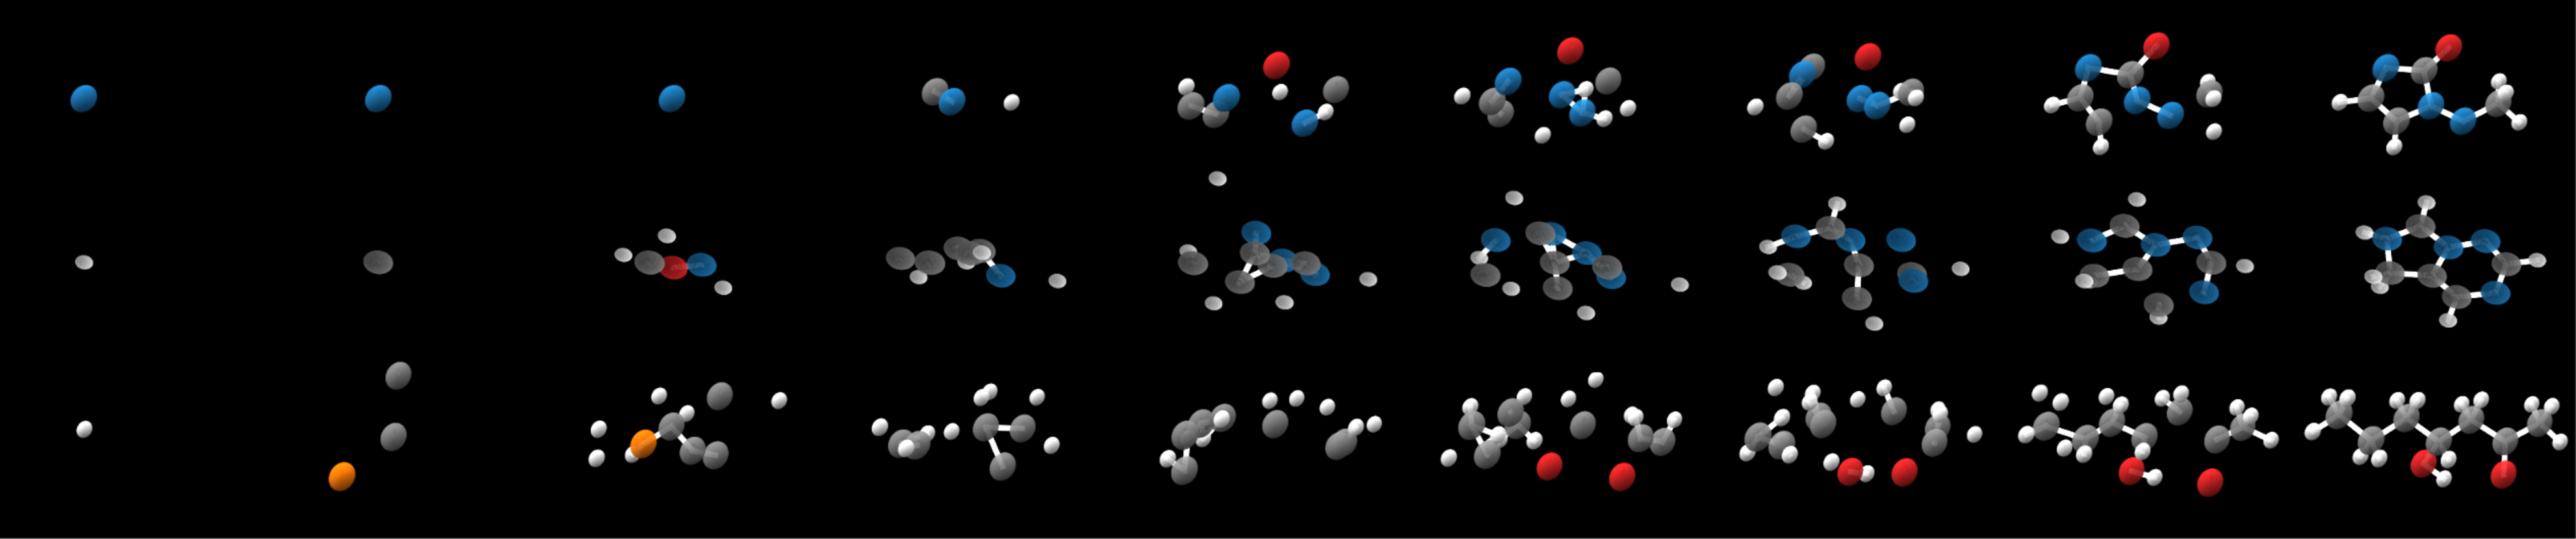
\includegraphics[width=\textwidth]{figs/tddm/genprog.pdf}
    \caption{Visualisation of the jump-diffusion backward generative process on molecules.}
    \label{fig:tddm-uncond_chain_vis}
\end{figure}


\begin{table}[t]
\caption{Sample quality metrics for unconditional molecule generation. An atom is stable if it has the correct valency whilst a molecule is considered stable if all of its atoms are stable. Molecular validity is measured using RDKit \cite{rdkit}. All methods use 1000 simulation steps and draw 10000 samples.}
\label{tab:uncond_mol}
\centering
\begin{tabular}{@{}lccc@{}}
\toprule
Method & \shortstack{\% Atom \\ Stable ($\uparrow$)} & \shortstack{ \% Molecule \\ Stable ($\uparrow$)} & \% Valid ($\uparrow$) \\ \midrule
FDDM \cite{hoogeboom2022equivariant} & $\mathbf{98.7}$ & $82.0$ & $91.9$  \\ \midrule
TDDM (ours) & $98.3$  & $\mathbf{87.2}$ & $\mathbf{92.3}$ \\
TDDM, const $\smash{\forwardrate_t}$ & $96.7$ & $79.1$ & $86.7$ \\
TDDM, $\smash{\forwardrate_{t<0.9T} = 0}$ & $97.7$ & $82.6$ & $89.4$ \\
TDDM w/o \cref{prop:backwardrateparam} & $97.0$ & $66.9$ & $87.1$ \\ \bottomrule
\end{tabular}
\end{table}
 

\subsubsection{Trans-Dimensional Diffusion Guidance}
\label{sec:mol_diff_guide}
We now apply diffusion guidance to our unconditional model in order to generate molecules that contain a certain number of desired atom types, e.g. 3 carbons or 1 oxygen and 2 nitrogens. The distribution of molecule sizes changes depending on these conditions. We generate molecules conditioned on these properties by using the reconstruction guided sampling approach introduced in \cite{ho2022video}. This method augments the score $s_{t}^\theta(\mX_t)$ such that it approximates $\nabla_{\rvx_t} \log p_{t}(\mX_t | y)$ rather than $\nabla_{\rvx_t} \log p_{t}(\mX_t)$ (where $y$ is the conditioning information) by adding on a term approximating $\nabla_{\rvx_t} \log p_{t}(y | \mX_t)$ with $p_t(y | \mX_t) = \sum_{n_0} \int_{\rvx_0} p(y | \mX_0) p_{0|t}(\mX_0 | \mX_t) \rmd \rvx_0 $. This guides $\rvx_t$ such that it is consistent with $y$. Since $\smash{\backwardrate_t^\theta(\mX_t)}$ has access to $\rvx_t$, it will cause $n_t$ to automatically also be consistent with $y$ without the user needing to input any information on how the conditioning information relates to the size of the datapoints. We give further details on diffusion guidance in \cref{sec:tddm-ApdxDiffGuide}.

\begin{table}[tb]
\caption{Conditional Molecule Generation for 10 conditioning tasks that each result in a different dimension distribution. We report dimension error as the average Hellinger distance between the generated and ground truth dimension distributions for that property as well as average sample quality metrics. Standard deviations are given across the 10 conditioning tasks. We report in bold values that are statistically indistinguishable from the best result at the $5\%$ level using a two-sided Wilcoxon signed rank test across the 10 conditioning tasks.}
\label{tab:cond_mol}
\centering
\begin{tabular}{@{}lcccc@{}}
\toprule
Method & \shortstack{Dimension \\ Error ($\downarrow$) } & \shortstack{ \% Atom \\ Stable ($\uparrow$)} & \shortstack{\% Molecule \\ Stable ($\uparrow$)} & \% Valid ($\uparrow$) \\ \midrule
FDDM & $0.511 {\scriptstyle \pm 0.19}$ & $93.5 {\scriptstyle \pm 1.1}$ & $31.3 {\scriptstyle \pm 6.3}$ & $65.2 {\scriptstyle \pm 10.3}$ \\ \midrule
TDDM  & $\mathbf{0.134 {\scriptstyle \pm 0.076}}$ & $93.5 {\scriptstyle \pm 2.6}$ & $\mathbf{59.1 {\scriptstyle \pm 11}}$ & $\mathbf{74.8 {\scriptstyle \pm 9.3}} $ \\
 TDDM, const $\smash{\forwardrate_t}$ & $0.226 {\scriptstyle \pm 0.17}$ & $88.9 {\scriptstyle \pm 4.8}$   & $43.6 {\scriptstyle \pm 15}$ & $63.4 {\scriptstyle \pm 14}$ \\
 TDDM, $\smash{\forwardrate_{t<0.9T} = 0}$&  $0.390 {\scriptstyle \pm 0.38}$& $\mathbf{95.0 {\scriptstyle \pm 2.1}}$& $\mathbf{61.7 {\scriptstyle \pm 17}}$ & $\mathbf{77.8 {\scriptstyle \pm 13}} $ \\
 TDDM w/o \cref{prop:backwardrateparam} & $0.219 {\scriptstyle \pm 0.12} $ & $\mathbf{93.8 {\scriptstyle \pm 3.2}}$ & $55.0 {\scriptstyle \pm 19}$ & $73.8 {\scriptstyle \pm 13}$  \\ \bottomrule
\end{tabular}
\end{table}

We show our results in \cref{tab:cond_mol}. In order to perform guidance on the FDDM baseline, we implement the model from \cite{hoogeboom2022equivariant} in continuous time and initialise the dimension from the empirically observed dimension distribution in the dataset.  This accounts for the case of an end user attempting to guide a unconditional model with access to no further information. We find that TDDM produces samples whose dimensions much more accurately reflect the true conditional distribution of dimensions given the conditioning information.
The $\forwardrate_{t<0.9T} = 0$ ablation on the other hand only marginally improves the dimension error over FDDM because all dimensions are added in the generative process at a time when $\mX_t$ is noisy and has little relation to the conditioning information. This highlights the necessity of allowing dimensions to be added throughout the generative process to gain the trans-dimensional diffusion guidance ability. The ablation with constant $\forwardrate_t$ has increased dimension error over TDDM as we find that when $\forwardrate_t > 0$ for all $t$, $\backwardrate_t^\theta$ can become very large when $t$ is close to 0 when the model has perceived a lack of dimensions. This occasionally results in too many dimensions being added hence an increased dimension error. Not using the \cref{prop:backwardrateparam} parameterisation also increases dimension error due to the increased difficulty in learning $\backwardrate_t^\theta$.

\begin{figure}[t]
    \centering
    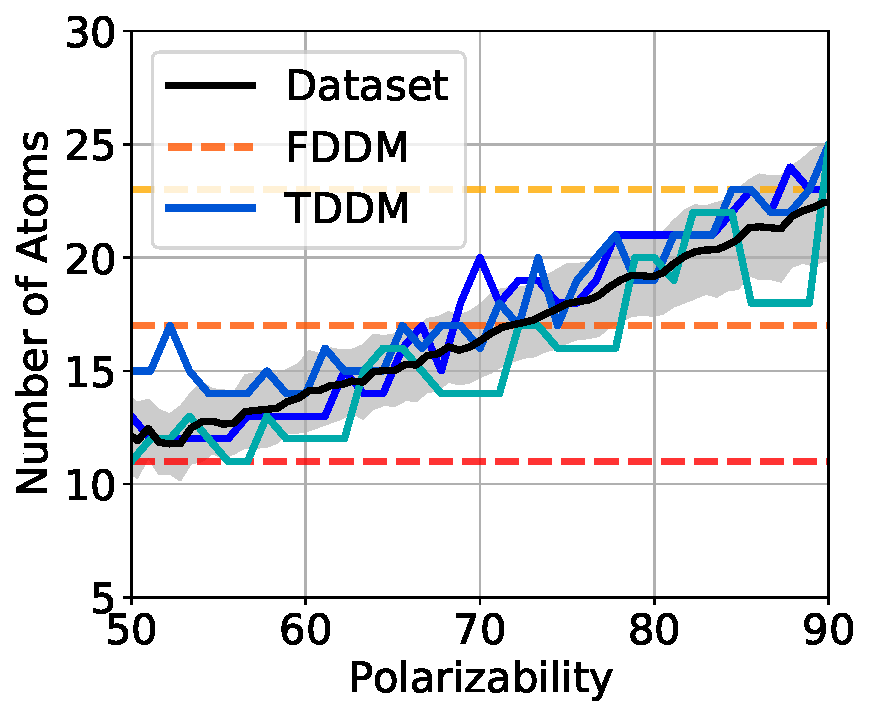
\includegraphics[width=0.45\textwidth]{figs/tddm/polarizability_vs_num_atoms.pdf}
    \caption{Number of atoms versus polarizability for $3$ interpolations with fixed random noise. The dataset mean and standard deviation for the number of atoms is also shown. FDDM interpolates entirely in a fixed dimensional space hence the number of atoms is fixed for all polarizabilities.}
    \label{fig:tddm-interp_plot}
\end{figure}

\subsubsection{Trans-Dimensional Interpolation}
\label{sec:mol_interp}
Interpolations are a unique way of gaining insights into the effect of some conditioning parameter on a dataset of interest.
To create an interpolation, a conditional generative model is first trained and then sampled with a sweep of the conditioning parameter but using fixed random noise \cite{hoogeboom2022equivariant}.
The resulting series of synthetic datapoints share similar features due to the fixed random noise but vary in ways that are very informative as to the effect of the conditioning parameter. 
Attempting to interpolate with an FDDM is fundamentally limited because the entire interpolation occurs in the same dimension which is unrealistic when the conditioning parameter is heavily correlated with the dimension of the datapoint. We demonstrate this by following the setup of \cite{hoogeboom2022equivariant} who train a conditional FDDM conditioned on polarizability.
Polarizability is the ability of a molecule's electron cloud to distort in response to an external electric field \cite{modernphysicalorganicchemistry} with larger molecules tending to have higher polarizability. To enable us to perform a trans-dimensional interpolation, we also train a conditional version of our model conditioned on polarizability. An example interpolation with this model is shown in \cref{fig:tddm-interp}. We find that indeed the size of the molecule increases with increasing polarizability, with some molecular substructures e.g.~rings, being maintained across dimensions.
We show how the dimension changes with polarizability during 3 interpolations in \cref{fig:tddm-interp_plot}. We find that these match the true dataset statistics much more accurately than interpolations using FDDM which first pick a dimension and carry out the entire interpolation in that fixed dimension.

\begin{figure}[t]
    \centering
    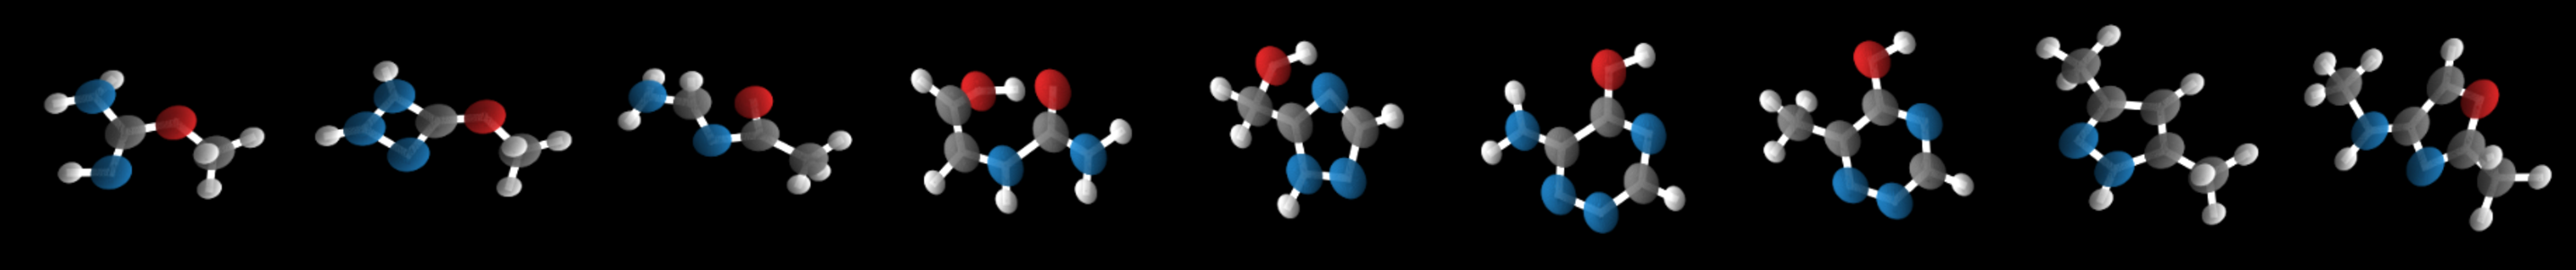
\includegraphics[width=\textwidth]{figs/tddm/small_interp_bright.pdf}
    \caption{Sequence of generations for linearly increasing polarizability from $39 \, \text{Bohr}^3$ to $66 \, \text{Bohr}^3$ with fixed random noise. Note how molecular size generally increases with polarizability and how some molecular substructures are maintained between sequential generations of differing dimension. For example, between molecules 6 and 7, the single change is a nitrogen (blue) to a carbon (grey) and an extra hydrogen (white) is added to maintain the correct valency.}
    \label{fig:tddm-interp}
\end{figure}



\subsection{Video}

We finally demonstrate our model on a video modelling task. Specifically we model the RoboDesk dataset~\citep{tian2023control}, a video benchmark to measure the applicability of video models for planning and control problems. The videos are renderings of a robotic arm~\citep{kannan2021robodesk} performing a variety of different tasks including opening drawers and moving objects.
We first train an unconditional model on videos of varying length and then perform planning by applying diffusion guidance to generate videos conditioned on an initial starting frame and a final goal frame \cite{janner2022diffuser}. The planning problem is then reduced to ``filling in'' the frames in between. Our trans-dimensional model automatically varies the number of in-filled frames during generation so that the final length of video matches the length of time the task should take, whereas the fixed dimension model relies on the unrealistic assumption that the length of time the task should take is known before generation.

We model videos at $32 \times 32$ resolution and with varying length from $2$ to $35$ frames. For the network backbone, we use a UNet adapted for video \cite{harvey2022flexible}. In contrast to molecular point clouds, our data is no longer permutation invariant hence $A_t^\theta(\yadd, i | \mX_t)$ includes a prediction over the location to insert the new frame. Full experimental details are provided in \cref{sec:tddm-ExperimentDetails}.
We evaluate our approach on three planning tasks, holding stationary, sliding a door and pushing an object. An example generation conditioned on the first and last frame for the slide door task is shown in \cref{fig:tddm-video_example}, with the model in-filling a plausible trajectory. We quantify our model's ability to generate videos of a length appropriate to the task in \cref{tab:video_results} finding on all three tasks we generate a more accurate length of video than FDDM which is forced to sample video lengths from the unconditional empirically observed length distribution in the training dataset.

\definecolor{videored}{HTML}{f00606}
\definecolor{videoblue}{HTML}{4b4bfc}

\begin{figure}[t]
    \centering
    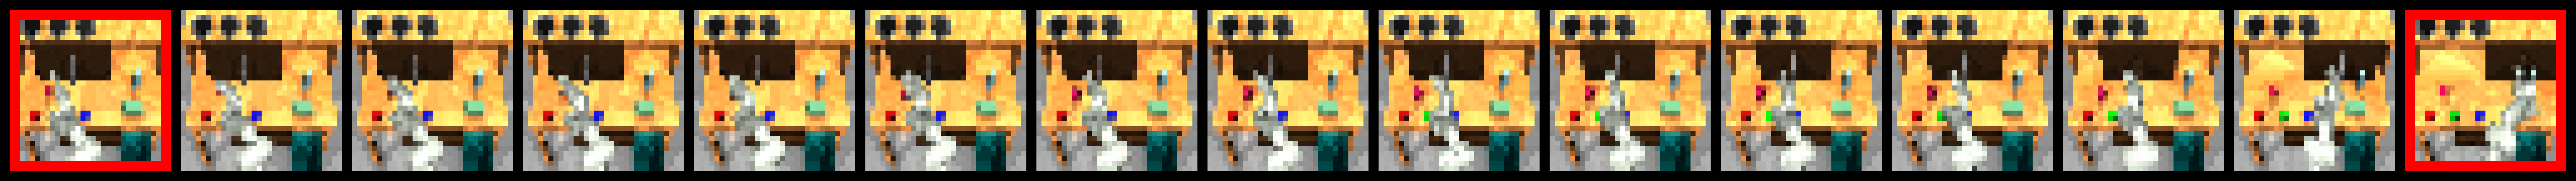
\includegraphics[width=\textwidth]{figs/tddm/21-1-padded_red_big.png}
    \caption{A sample for the slide door task conditioned on the first and last frame ({\color{red} highlighted}).}
    \label{fig:tddm-video_example}
\end{figure}

\begin{table}[t]
     \centering
   \caption{Dimension prediction mean absolute error for three planning tasks with standard deviations estimated over 45 samples.}
   \begin{tabular}{@{}lcccc@{}}
     \toprule
     Method & Stationary ($\downarrow$) & Slide Door ($\downarrow$) & Push Object ($\downarrow$) & Average ($\downarrow$)   \\ \midrule
     FDDM & $14.16 {\scriptstyle \pm 1.41}$ & $13.39 {\scriptstyle \pm 1.34}$ & $17.06 {\scriptstyle \pm 1.47}$ & $14.87$ \\
     TDDM & $\mathbf{9.70 {\scriptstyle \pm 0.99}}$ & $\mathbf{11.47 {\scriptstyle \pm 0.74}}$ & $\mathbf{15.43 {\scriptstyle \pm 0.90}}$ & $\mathbf{12.2}$ \\ \bottomrule
   \end{tabular}
   \label{tab:video_results}
\end{table}
